\chapter{Kamery zdarzeniowe}
\label{cha: KameryZdarzeniowe}

W niniejszym rozdziale przedstawiono opis kamer zdarzeniowych. Przedstawiono główne różnice względem tradycyjnych czujników jak i sposoby przetwarzania danych z nich pochodzących. Zarysowano krótko historię ich powstania oraz komercyjną dostępność najpopularniejszych modeli. Na końcu przedstawiono analizę bibliotek ułatwiających pracę z nimi poprzez przykładowo możliwość przetworzenia ciągu wideo z kamery tradycyjnej na zdarzenia oraz udostępnione publicznie zbiory danych mogące służyć do testowania zaimplementowanych algorytmów.
\section{Opis urządzeń}
\label{sec:OpisUrzadzen}

    \subsection{Krótka historia}
    \label{subsec:historia}
    
    Historia kamer zdarzeniowych zaczyna się w roku 1986. Wtedy to właśnie doktorantka Misha Mahowald z firmy Calltech zaczyna pracę z profesorem Carver Mead`em nad problemem stereowizji z punktu widzenia zarówno aspektu inżynierskiego jak i biologicznego. Celem było stworzenie systemu wizyjnego działającego w sposób jak najbardziej zbliżony do ludzkiego oka. Został on osiągnięty wraz z publikacją przez nich w roku 1991 artykułu w ''Scientific American'' opisującego działanie ich sprzętu - siatkówki silikonowej (ang.\emph{Silicon Retina}). Był to pierwszy krok w rozwoju nowego rodzaju czujnika, czyli kamery zdarzeniowej (ang \emph{Event Camera}). Przez kolejne dekady opracowane zostały trzy różne typy czujników, tj. DAVIS, DVS oraz ATIS. Pierwszy czujnik tego typu do komercyjnego użytku trafił w roku 2008  i był to model DVS128 wprowadzony przez firmę IniVation. W ciągu kolejnych lat do tego grona dołączyli kolejni producenci tacy jak Prophesee (rok 2011), Samsung (rok 2017), CelePixel (rok 2017) oraz Insightness Rino 3 (rok 2018) (\ref{fig:Komercyjne})
    
    
    \subsection{Porównanie do klasycznych kamer}
    \label{subsec:Porownanie}
    
    Kamery zdarzeniowe to asynchroniczne czujniki które reagują na dynamiczne zmiany oświetlenia danej sceny. Danymi na których operują są zdarzenia (ang \emph{events}) oznaczające zmiany oświetlenia jakie zaszły w rozpatrywanym pikselu matrycy. Wyjściem takich kamer są więc sekwencje zdarzeń, z których każde odpowiada zmianie jasności o określony próg liczony w skali logarytmicznej w danych okresie czasu. Odpowiada to sposobowi w jaki ludzkie oczy odbierają świat zewnętrzny. Jest to całkowicie odmienny sposób działania w porównaniu do dotychczas stosowanych kamer, które generowały kolejne ramki obrazu co określony czas definiowany przez ich wewnętrzny zegar np. 40 na sekundę (40 fps ang. \emph{frames per second}).
    Każdy piksel zapamiętuje intensywność padającego światła w chwili wysyłania zdarzenia a następnie sprawdza czy w kolejnych chwilach czasowych ilość ta zwiększyła bądź też zmniejszyła się o z góry zadaną przez użytkownika wartość. Kiedy dochodzi do takiej sytuacji wysyła informację o zdarzeniu w formie zawierającą informację o swoim położeniu \emph{x,y}, czasie \emph{t} jak i wartości \emph{p} - zmiana jasności w górę bądź w dół. Ważnym aspektem tych czujników jest ich zależność od zdarzeń - ilość informacji jakie wysyłają nie jest stała, ale zależna od zmian oświetlenia. Im częściej ona następuje tym więcej zdarzeń zostanie wygenerowanych. Na Rysunku \ref{fig:events} przedstawiono z lewej strony obraz uzyskany kamerą standardową, natomiast po lewej jego prezentację w przestrzeni zdarzeń uzyskaną przy pomocy symulatora ESIM.\\
    
    \begin{figure}[h]
        \centering
        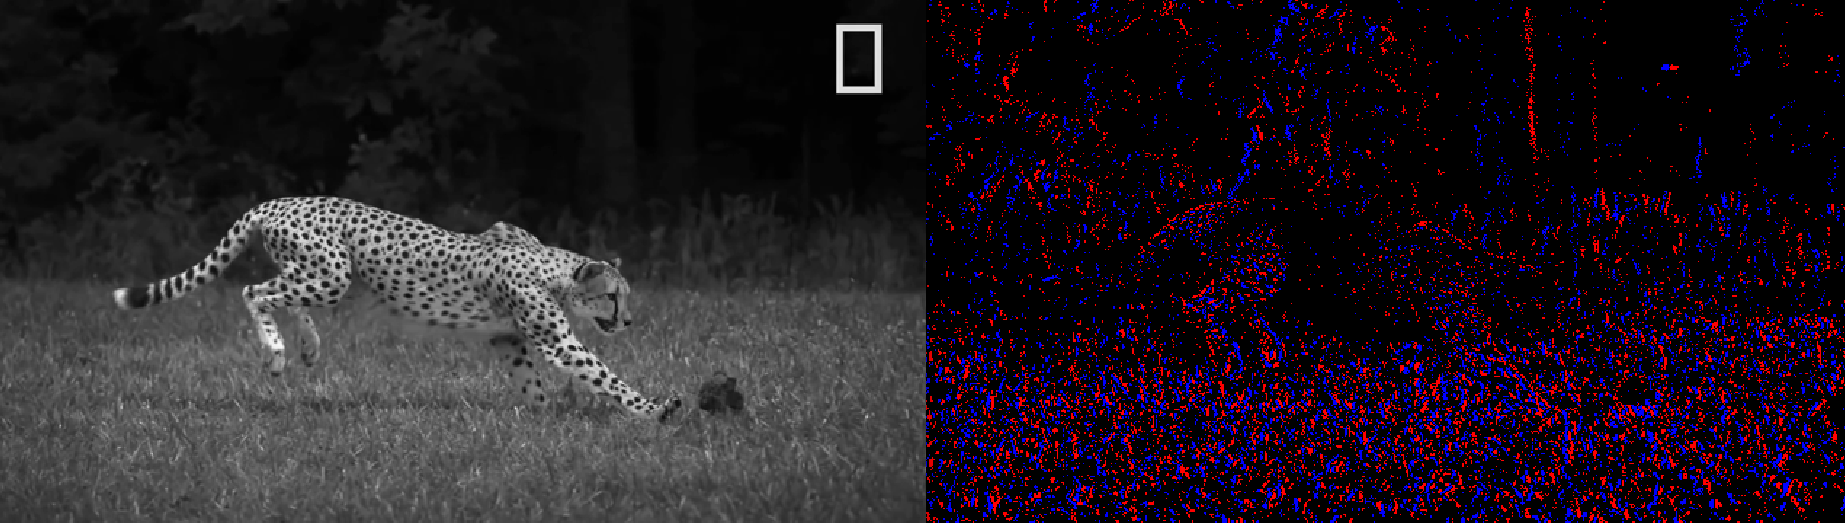
\includegraphics[width=\textwidth]{Codes/ESIM_test/screenshot2.png}
        \caption{Porównanie standardowej ramki obrazu (lewej strona) oraz zdarzeń (prawa strona) - wykorzystano symulator ESIM}
        \label{fig:events}
    \end{figure}
        
    \indent W porównaniu do tradycyjnych kamer, kamery zdarzeniowe posiadają szereg zalet, takich jak(\cite{Sourvey}):
    \begin{itemize}
        \item   Wysoka Rozdzielczość Czasowa (ang. \emph{Temporal Resolution}) - Badanie zmian jasności padającego na piksel jest szybka, z kolei odczyt danych z kamery odbywa się z częstotliwością 1 MHz. Dzięki temu kamery zdarzeniowe są w stanie wykryć bardzo szybki ruch przedmiotów bez
        zachodzenia zjawiska rozmycia w ruchu (ang \emph{Motion Blur})
        
        \item  Mała Latencja (ang. \emph{Latency}) - Każdy piksel pracuje asynchronicznie do reszty na matrycy wobec czego nie zachodzi konieczność czekania na dane od pozostałych. Mogą więc być bardzo szybko wysyłane - latencja liczona jest w milisekundach w zastosowaniach praktycznych.
        
        \item Małe zużycie energii (ang. \emph{Power}) - Kamery zdarzeniowe transmitują jedynie zmiany jasności, wobec czego nie ma  przesyłanych żadnych zbędnych danych. Energia jest więc wykorzystywana tylko do przetwarzania pikseli które uległy zmianie. Zużycie energii wynosi około 10 mW.
        
        \item Duża Rozdzielczość Dynamiczna (ang. \emph{Dynamic Range}) - Wysokiej jakości tradycyjne kamery osiągają 60dB, podczas gdy kamery zdarzeniowe osiągają wartości ponad 2 razy większe. Pozwala to na bezproblemową akwizycję danych zarówno za dnia jak i w nocy. 
        
    \end{itemize}

    Bardzo ważnym aspektem na który należy zwrócić uwagę, jest fakt iż pomimo swoich niewątpliwych zalet nad kamerami standardowymi, kamera zdarzeniowa generuje dane w sposób nowatorski, całkowicie odmienny od dotychczas stosowanych.Nie działają one na ramkach a na zdarzeniach, liczba danych jest zależna od dynamiki sceny oraz nie posiadają one bezpośrednich informacji na temat jasności pikseli a jedynie na temat ich zmiany.Prowadzi to do konieczności utworzenia nowych algorytmów przetwarzania obrazu bądź też dostosowania już istniejących do innego typu danych wejściowych.
    
    \subsection{Model generowania zdarzeń}
    \label{subsec:Model}
    Jak wspomniano w \ref{subsec:Porownanie} kamery zdarzeniowe reagują na dynamiczne zmiany oświetlenia w przetwarzanej scenie. Składają się z siatki działających od siebie niezależnie pikseli które reagują na progowe zmiany oświetlenia w skali logarytmicznej \(L = log(I) \), gdzie I oznacza jasność. Przy założeniu braku szumu zdarzenie  \(e_k = (X_k, t_k, p_k) \) o wartości \(p_k \in \{-1, 1\}\) jest generowane w punkcie \( X_k = (x_k, y_k) \) w punkcie czasowym \(t_k\) w którym poziom jasności padający na punkt przekroczył zadany próg o \(\pm\ C > 0\):
        
    \begin{equation}
    \label{eq:1}
        \Delta L(X_k, t_k) =  L(X_k, t_k) -  L(X_k, t_k- \Delta t_k)
    \end{equation}
    
    \begin{equation}
    \label{eq:2}
        \Delta L(X_k, t_k) = p_k C
    \end{equation}
gdzie \(\Delta t_k = t_k - t_{k-1}\) to czas jaki minął od czasy wystąpienia poprzedniego zdarzenia \(e_{k-1}\)
    
    \subsection{Typy urządzeń}
    \label{subsec:TypyUrzadzen}
    Jak wspomniano w \ref{subsec:historia} pierwszy istniejący prototyp kamery zdarzeniowej wykonano przez duet Mahowald oraz Mead w latach 1986-1992. Ich projekt został nagrodzony nagrodą Clauser`a przyznawaną dla wybitnych prac dyplomowych doktoranckich. Był to jednak jedynie pierwszy krok w rozwoju tego typu czujników i posiadał wady. Wśród nich wymienić można zbyt dużą wielkość pikseli uniemożliwiającą praktyczne zastosowanie urządzenia czy też znaczące różnice pomiędzy odpowiedziami różnych pikseli. W kolejnych latach jednak nastąpił jednak skok rozwojowy tych urządzeń doprowadzając do powstanie sensorów lepszej jakości, wśród których najpopularniejsze konstrukcje to DVS (ang. \emph{Dynamic Vision Sensor}), ATIS (ang. \emph{Asynchronous Time Based Image Sensor}) oraz DAVIS (ang. \emph{Dynamic and Active Pixel Vision Sensor}). Dwa ostatnie jednak stanowią rozszerzenie DVS i z racji iż zawierają jego komórki nazwy DVS można używać się do określenia każdego typu kamery zdarzeniowej bez względu na typ budowy.\
    
    \indent Podstawową i pierwszą zastosowaną komercyjnie konstrukcję stanowi DVS. Bazuje ona na typie  krzemowej siatkówki w której fotoreceptor zbierający dane w czasie rzeczywistym jest połączony poprzez swoją pojemność do układu odczytującego resetującego swoje dane za każdym odczytem zawartości piksela.\ 
    
    \indent Kolejny typ stanowi ATIS. Był jedną z odpowiedzi na podstawowy problem DVS - braku informacji statycznych dotyczących sceny jak przykładowo wartość absolutna poziomu jasności. Na jego matrycy umieszczone są piksele zawierające pomniejsze piksele typy DVS które uruchamiają inne pomniejsze piksele, ich zadaniem jest z kolei odczytywać absolutną wartość poziomu światła. Problemem układu tego typu wielkość pikseli, co najmniej dwa razy większa niż w DVS.\
    
    \indent Ostatni typ stanowi DAVIS. Na jego matrycy piksele zawierają piksele DVS oraz APS (ang. \emph{Active Pixel Sensor}). Ze względu na współdzielenie fotodiod rozmiar pikseli jest znacznie mniejszy niż w przypadku ATIS. Ograniczeniem jednak jest mniejsza rozdzielczość dynamiczna wynosząca 55 dB.
    
    
    
    \subsection{Dostępność komercyjna}
    \label{subsec:Dostepnosc}
    W Tabeli \ref{fig:Komercyjne} przedstawiono dostępne komercyjnie kamery zdarzeniowe od różnych producentów.
    
   \begin{figure}[h]
       \centering
       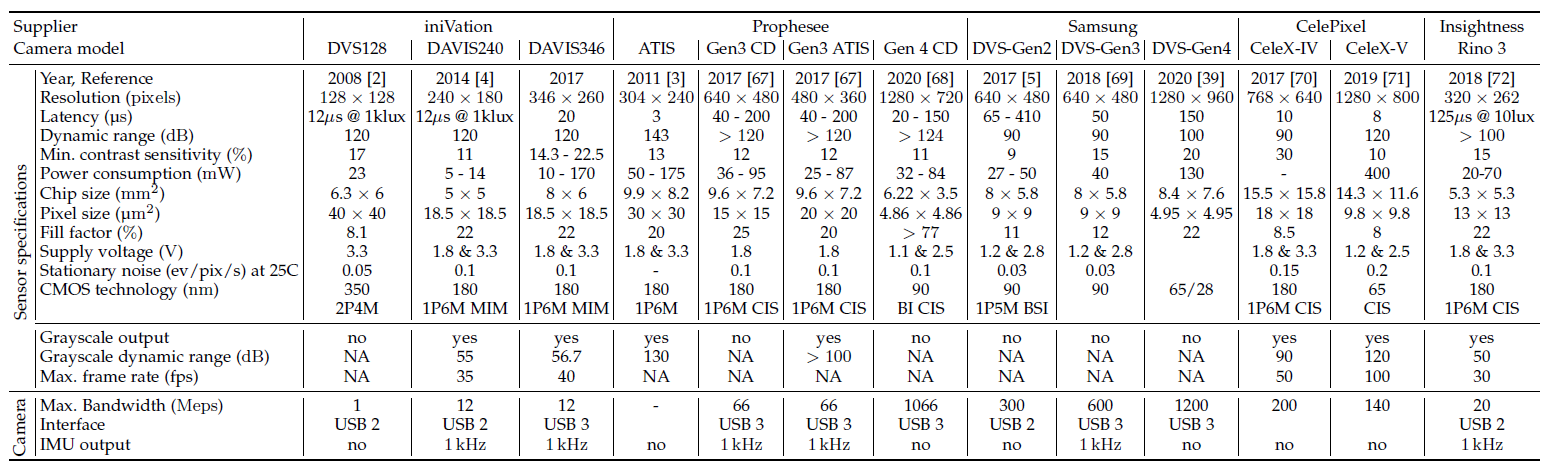
\includegraphics[width=\textwidth]{Thesis/Literatura/Events/KamryZdarzenioweNaRynku.PNG}
       \caption{Kamery zdarzeniowe dostępne komercyjnie \cite{Sourvey}}
       \label{fig:Komercyjne}
   \end{figure}
   
   Jak można zauważyć, pierwszą komercyjnie dostępną konstrukcją była DVS128 firmy iniVation. Zwrócić należy uwagę na jej bardzo małą rozdzielczość - 128 x 128. Było to za mało na zastosowanie jej w celach praktycznych. Na przestrzeni kolejnych lat wypuszczane konstrukcje charakteryzowały się większymi rozdzielczościami aż do modelu DVS-Gen4 Samsunga - 1280 x 960. Kierunkiem w jakim podążył rozwój było również systematyczne zmniejszanie latencji oraz dodawanie dodatkowych elementów - wyjścia w skali szarości oraz IMU (ang. \emph{Inertial Measurement Unit}) - nawigacji inercjalnej.\\
   
   Na drodze rozwoju kamer zdarzeniowych stoi kilka problemów. Jednym z nich jest kwestia organizacyjna producentów - nie istnieją uniwersalne i powszechnie stosowane metody testowania takiego sprzętu. Nie został wyspecyfikowany standard dla tego sprzętu wobec czego porównywanie kamer różnych producentów nie musi w pełni odzwierciedlać różnic rzeczywistych.
   Niewielka (w porównaniu do kamery tradycyjnych) rozdzielczość wynika z wielkości pikseli na matrycy. Z racji na swoją asynchroniczność układ zajmuje dużo przestrzeni co przekłada się również na koszta poprzez konieczność zastosowania sporej ilości krzemu do produkcji. Jednym z potencjalnych rozwiązań tego problemu może być odejście od pełnej asynchroniczności pikseli do częściowej. Kolejnym problemem z jakim mierzą się kamery zdarzeniowe jest współczynnik wypełnienia (ang. \emph{Fill Factor}). Jest to stosunek powierzchni fotoczułej piksela do jego całkowitej powierzchni. Przykładowo konstrukcja DAVIS346 posiada współczynnik równy 20\%. Oznacza to, że tylko 1/5 wszystkich fotonów padająca na jej pojedynczy piksela zostanie zarejestrowana. Z punktu widzenia wydajności systemu jest to wartość niezadowalająca. Obejście tego problemu może się odbyć na co najmniej dwa sposoby. Po pierwsze można zastosować mikrosoczewki skupiające światło na fotodiodzie. Innym rozwiązaniem jest technika \emph{BSI}(ang. \emph{Back-side Illumination}). Polega ona na odwróceniu kolejności elementów w krzemie w taki sposób aby był on oświetlany niejako od tyłu. W ten sposób cały obszar piksela może zbierać informacje o oświetleniu. To rozwiązanie generuje jednak dodatkowe koszty. Stanowią one największą przeszkodę wykorzystania komercyjnego kamer zdarzeniowych. Koszt zakupu sprzętu to co najmniej kilka tysięcy złotych. Na taki stan rzeczy składają się w większości wspomnianie wcześniej kwestie - duża ilość krzemu, techniki oświetlenia fotodiody czy też jednorazowe koszta zaprojekowania konstrukcji. Wraz z upowszechnieniem technologii spodziewać należy się jednak spadku cen.
    
    
    \subsection{Przetwarzanie danych}
    \label{subsec:Przetwarzanie}
    
    Dla wykorzystania kamer zdarzeniowych w praktyce najważniejszym problemem jest odpowiednie przetwarzanie pochodzących z niej zdarzeń. Nie istnieje jednak jedna uniwersalna metoda radzenia sobie z tym zagadnieniem i wiele zależy od celu implementowanej aplikacji. Ogromną rolę odgrywa tutaj również aspekt czasowy z racji iż ilość danych nie stała i ich ilość w czasie zależy od dynamiki sceny. Algorytmy przetwarzania można podzielić na kilka kategorii w zależności chociażby od ilości przetwarzanych elementów czy też od implementacji na bazie algorytmu bądź też danych. W tej pierwszej kategorii podział odbywa się na przetwarzanie każdego zdarzenia z osobna  albo w paczkach zdarzeń. Wprowadza to dodatkową latencję do całego systemu. Z kolei rozróżnienie na bazie implementacji wprowadza rozróżnienie pomiędzy klasyczne metody wizyjne dostosowane do kamer zdarzeniowych a coraz popularniejsze uczenie przy pomocy sieci neuronowych, głównie impulsowych SNN (ang. \emph{Spiking neural Network}).\\
    Przetworzone zdarzenia często są przekształcane w alternatywne reprezentacje w celach szybszej bądź też efektywniejszej dalszej pracy z nimi. Poza standardowymi pojedynczymi zdarzeniami bądź paczkami zdarzeń wyróżnić można między innymi (za \cite{1}):
    \begin{itemize}
    
        \item Ramka ze zdarzeniami (ang. \emph{Event Frame}) - Jest to proste zrzutowanie zdarzeń na przestrzeń 2D z ukazaniem polaryzacji tak jak na Rys \ref{fig:events}. Takie zdjęcie można przekazać dalej do klasycznego algorytmu wizyjnego, jednakże w takim rozwiązaniu tracimy częściowo informację na temat czasy wystąpienia danego zdarzenia, musimy bowiem w danym oknie czasowym przeprowadzić ich kumulację. Obrazy tego typu są jednak dość intuicyjne do zrozumienia przez człowieka gdyż dobrze ukazują krawędzie obiektów rozpatrywanej sceny.
        
        \item Powierzchnia czasowa (ang. \emph{Time Surface}) - Jest to mapa 2D w której każdy piksel przechowuje pojedynczą informację o czasie wystąpienie ostatniego zdarzenia w tej lokalizacji. Wartość w tym pikselu jest zależna od funkcji opisującej historię jego ruchu - im większa tym bardziej aktualny był jego ruch. W przełożeniu na klasyczne komputerowe przetwarzanie obrazu nazywamy to obrazem historii ruchu (ang. \emph{Motion History Image}). Dzięki temu łatwiej można odróżnić aktualne zdarzenia od poprzednich.
        
        \item Przestrzeń 3D (ang. \emph{3D Point Set}) - Jest to przedstawienie zdarzeń na układzie 3D reprezentującym ich pozycję na powierzchni kamery oraz czas wystąpienia - \((x_k, y_k, t_k)\) 
        
        \item Siatka wokseli (ang. \emph{Voxel Grid}) - Podobnie jak poprzednik wykorzystuje ona przestrzeń 3D tutaj jednak w celu ukazania histogramu zdarzeń w którym każdy woksel (trójwymiarowy piksel) reprezentuje piksel oraz przedział czasowy.
        
        
        \item Ramka z kompensacją ruchu (ang. \emph{Motion-Compensated Event Image}) - Jest to sposób reprezentacji w którym w określony sposób niweluje się ruch krawędzi obiektów w scenie. Dzięki temu uzyskuje się obraz przedstawiający ich krawędzie. Jest on łatwiejszy do odczytania przez człowieka niż zwykła ramka ze zdarzeniami. 
        
        \item Zrekonstruowana ramka (ang. \emph{Reconstructed Images}) - Przy pomocy osobnych algorytmów rekonstrukcyjnych możliwe jest przetworzenie ciągu zdarzeń na obraz w skali szarości, taki jaki można uzyskać przy pomocy standardowej kamery.
    \end{itemize}
    

\section{Analiza bibliotek}
\label{sec:Biblioteki}

    \subsection{v2e}
    \label{subsec:v2e}
    
    V2e jest dziełem pracy prowadzonej przez uniwersytet w Zurichu. Jest to narzędzie napisane w języku Python pozwalające na przetworzenie standardowej sekwencji wideo na syntentyczny ciąg zdarzeń DVS. Przykładowy obraz uzyskany z dostarczonej przez twórców oryginalnej sekwencji wideo przedstawiającej mecz tenisa przedstawiono na \ref{fig:v2e}
    
       \begin{figure}[h]
       \centering
       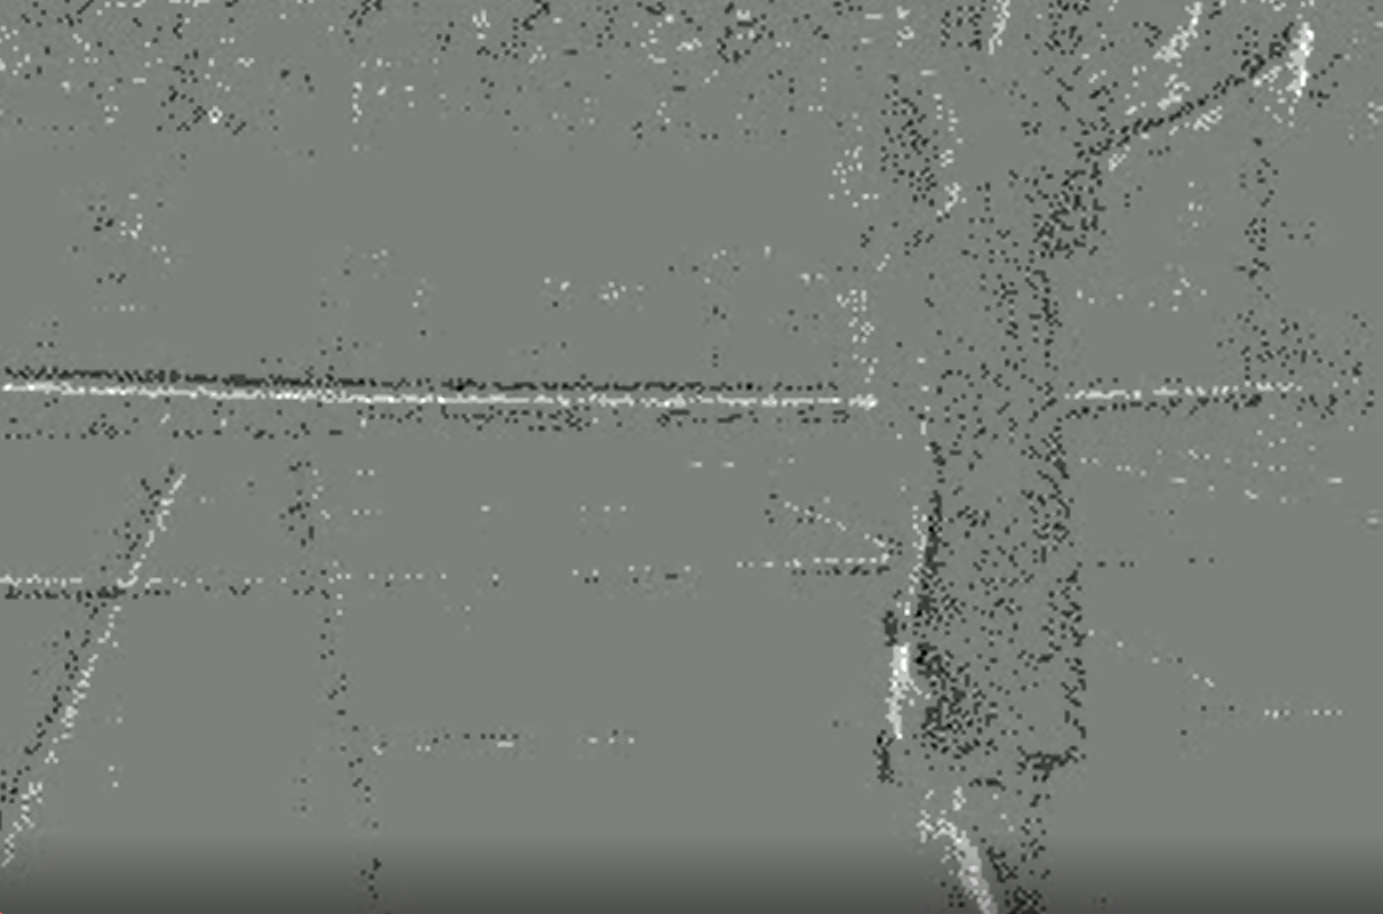
\includegraphics[width=\textwidth]{Codes/v2e_test/Tenis.PNG}
       \caption{Tenisista przetworzony przy pomocy v2e}
       \label{fig:v2e}
   \end{figure}
   
   Działanie programu można podzielić na następujące etapy (za \cite{v2e}):
   
   \begin{enumerate}
       \item Zmiana przestrzeni barw z RGB na luma - Początkowe wideo o długości \emph{T} zostaje przetworzone na ciąg \emph{M} ramek w przestrzeni barw luma.  Jest to przestrzeń barw reprezentująca jasność obrazu poprzez oddanie jego skali szarości. Każda ramka obrazu zostaje powiązana z chwilą czasową \( t_k\), gdzie \( t_0 = 0 < t_1 < ... < t_M = T \)
       
       \item Syntetyczne spowolnienie - Po zmianie przestrzeni barw następuje opcjonalna interpolacja ilości ramek przy użyciu syntentycznego spowolnienia ramek w celu zwiększenia rozdzielczości czasowej. Do tego celu używana jest głęboka sieć konwolucyjna \emph{Super-SloMo}. Przewiduje ona przepływ optyczny pomiędzy dwiema ramkami który to jest następnie używany do sztucznego wytworzenia nowych pomiędzy nimi z przypisaniem im chwil czasowych pomiędzy przetwarzanymi. Idealnym rozwiązaniem jest wytworzenie takich ilości ramek aby różnica w ruchu pomiędzy dwiema ramkami nie była większa niż jeden piksel.
       
       \item Mapowanie przestrzeni liniowej do logarytmicznej - W celu przejścia na przestrzeń logarytmiczną stosowaną przez kamery zdarzeniowe następuje mapowanie lin-log dla każdej pojedynczej ramki, jeżeli tylko wartość luma wynosi powyżej 20. Dla mniejszych wartości stosujemy mapowanie liniowe z wartości intensywności do przestrzeni logarytmicznej. Oznacza to, że małe wartości zostaną przekonwertowane w sposób liniowy zmniejszając kwantyzację szumu na wyjściu.
       
       \item Użycie filtru  - Rozdzielczość dynamiczna kamer zdarzeniowych jest duża, ale nie jest nieskończona. Konieczne jest więc ograniczenie rozdzielczości wartości syntetycznych poprzez zastosowanie dodatkowego filtru dolnoprzepustowego.
       
       \item Wygenerowanie zdarzeń - Na wyjściu poprzedniego punktu otrzymaliśmy przefiltrowaną wartość odzwierciedlającą wartość intensywności 
       światła padającego na rozpatrywany aktualnie piksel. Można więc zastosować znane już równanie \ref{eq:1}, przy założeniu, że wartości w chwili czasowej \( t_k - \Delta t\) są znane z poprzedniej iteracji. Jeżeli różnica ta jest wielokrotnością ustalonego odpowiednio progu zdarzenia dodatniego bądź też ujemnego (progi nie muszą być sobie równe) następuje wygenerowanie odpowiedniej ilości zdarzeń oraz zapamiętana zostaje nowa aktualna wartości intensywności. 
       
       \item Dodanie szumu - W celu lepszego oddania własności rzeczywistego układu kamery zdarzeniowej v2e generuje szum w oparciu o rozkład Poisson`a.
       
   \end{enumerate}
   
   Instalacja pakietu przebiega w sposób intuicyjny i prosty. API aplikacji pozwala na pracę zarówno z poziomu konsoli poprzez wywołanie odpowiednich argumentów bądź też przy pomocy GUI zaprojektowanego za pomocą pakietu \emph{Gooey}.
   
   
    
    \subsection{ESIM}
    \label{subsec:esim}
    Projekt ESIM (ang. \emph{Open Event Camera Simulator}) powstał w ramach pracy badawczej doktora Davide Scaramuzzy również na uniwersytecie w Zurychu. Celem było stworzenie nie tyle narzędzia do przekształcania standardowej sekwencji wideo na syntetyczne zdarzenia DVS, ale również stworzenie środowiska do implementacji oraz testowania aplikacji na nich bazujących. Projekt oparto na oprogramowaniu ROS (ang. \emph{Robotic Operating System}) w wersji Kinetic.
    
    Symulator ESIM opiera swoje działanie o dwa główne elementy (\cite{ESIM}):
    
    \begin{enumerate}
        \item Sensor ruchu (ang. \emph{Sensor trajectory}) - Reprezentuje on funkcję regularną \(\tau \) która mapuje każdą chwilę czasową \(t \) do pozycji sensora, jego skrętu oraz przyspieszenia.
        
        \item Silnik wyświetlania (ang. \emph{Rendering engine}), renderer - Jest to funkcja  \( R\) która mapuje każdą chwilę czasową \(t\) do wyrenderowanego obrazu albo irradiancji sceny dla obecnej pozycji sensora. Renderer jest parametryzowany poprzez środowisko, trajektorię sensora wewnątrz środowiska oraz konfigurację sensora. Środowisko kontroluje geometrię sceny jak i jej zmienność. Trajektoria sensora reprezentuje trajektorię kamery wewnątrz środowiska które może być generowane w czasie rzeczywistym na podstawie dynamicznego modelu robota i zestawu funkcji kontrolujących albo wyliczona wcześniej. Konfiguracja sensora reprezentuje konfigurację wirtualnego sensora na które składają się parametry zewnętrzne oraz wewnętrzne. Zawiera także parametry specyficzne dla sensora jak przykładowo próg \(C\) . Renderer dodatkowo wylicza także Pole Ruchu (ang. \emph{Motion Field Map}) czyli projekcję 3D relatywnych wektorów ruchu na przestrzeń 3D. Jest to pewnego rodzaju aproksymacja Przepływu Optycznego (ang. \emph{Optical Flow}). W ESIM używana jest do obliczania spodziewanej zmiany natężenia światła.
    \end{enumerate}
    
    W przeciwieństwie do V2e, które swoje działanie w dużej mierze opiera na rozmieszczeniu pikseli w taki sposób aby pomiędzy kolejnymi aproksymowanymi ramkami przemieszczenia były jak najmniejsze, ESIM opiera swoje działanie na zmianie jasności. Sprowadza się to do użycia rozwinięcia w szereg Taylora co pozwala uzyskać przewidywaną zmianę natężenia światła w danym pikselu \(x\), chwili czasowej \(t\) podczas danego wycinka czasu \(\Delta t\): \(\Delta \mathcal{L} \approx \frac{\delta \mathcal{L}(x;t_k)}{\delta t} \Delta t  \), gdzie \(\ \mathcal{L} \) to poziom jasności piksela. Korzystamy przy tym z informacji pozyskanych z pola ruchu.
    
    W celu lepszego odwzorowania działania prawdziwych kamer zdarzeniowych w ESIM zaimplementowany został również, podobnie jak w V2e, model szumu w oparciu o rozkład normalny.
    
    Poza standardowym przetwarzaniem wideo na ciąg syntetycznych zdarzeń ESIM oferuje również szereg innych możliwości poprzez różnego typu silniki wyświetlania. Jest to m.in. silnik OpenGLRenderer pozwalający na obsługę przestrzeni 3D. Przykład użycia z dostarczonych przez twórców próbek ukazano na rysunku \ref{fig:ESIM_3D}. Dolna jego część przedstawia ruch kamery z zaznaczonymi zdarzeniami na terenie z wypukłościami, natomiast górna część próbę ukazania jej w przestrzeni zdarzeń 3D.
    
    \begin{figure}
        \centering
        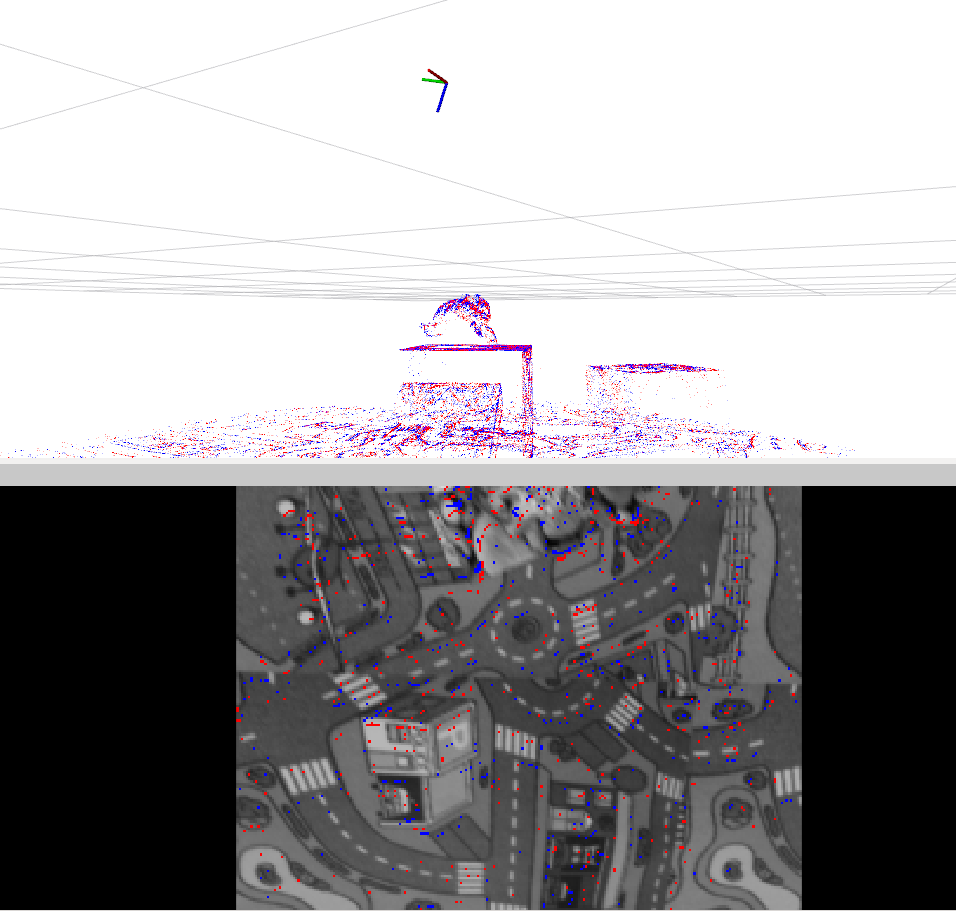
\includegraphics[width=\textwidth]{Codes/ESIM_test/3D_test.png}
        \caption{Możliwość silnika graficznego OpenGLRenderer symulatora ESIM - odtwarzanie zdarzeń w przestrzeni 3D}
        \label{fig:ESIM_3D}
    \end{figure}
    
    
    \subsection{Prophesee OpenEB}
    \label{subsec:openEB}
    Prophesee jest korporacją pochodzenia francuskiego zajmującą się projektowaniem oraz sprzedażą kamer zdarzeniowych jak i o oprogramowania do nich. W roku 2021 firma udostępniła otwartoźródłowe oprogramowanie OpenEB oraz biblioteki do języka Python mające umożliwić łatwiejszy start w tematach pracy na zdarzeniach ludziom nieobeznanym w tej tematyce do tej pory. {\color{red}{Więcej chwilowo trudno napisać bo Essentials nie działa, nikt nie wie dlaczego a Prophesee nie odpowiedziało mi na maila.}}

\section{Zbiory danych}
\label{sec:ZbioryDanych}

    \subsection{MVSEC}
    \label{subsec:mvsec}
    MVSEC (ang. \emph{The Multi Vehicle Stereo Event Camera Dataset}) jest dużą bazą danych zawierającą informacje stereowizyjne z kamer zdarzeniowych. Zgodnie z \cite{MVSEC} zawiera on następujące dane w formacie ROS:
    
    \begin{itemize}
        \item Zdarzenia, zdjęcia w skali szarości APS oraz pomiary IMU z lewej i prawej kamery DAVIS
        
        \item Zdjęcia oraz pomiary IMU z sensora VI
        
        \item Chmury punktów zebrane przy użyciu lidaru VLP-16
        
        \item Pozycje referencyjne ground truth dla lewej kamery zdarzeniowej
        
        \item Referencyjne mapy ground truth głębi zarówno dla prawej jak i lewej kamery zdarzeniowej przy pomocy metod opisanych w \cite{DBLP:journals/corr/abs-1802-06898}
    \end{itemize}
    
    Użytymi kamerami zdarzeniowymi była para kamer DAVIS m346B o rozdzielczości 346 na 260 pikseli. Cały zestaw sensorów został umieszczony na różnych obiektach: dronie (hexacopterze), samochodzie, motocyklu oraz w chwycie ludzkich dłoni. Kalibracje kamer wykonano przy użyciu toolboxa Kalibr z użyciem równoległego modelu dystorsji. 
    
    Dane w formacie ROS częściowo przeniesiono na łatwiejszy do obsługi poza ROS typ txt. Zawierają one niektóre sekwencje zdarzeń oraz tak jak w formacie ROS, pliki z parametrami kamer i macierzami potrzebnymi w procesach kalibracji. Niestety, ich format nie został opisany w dokumentacji projektu który wydaje się nie być już aktualizowany - ostatnie zmiany pochodzą z 2018 roku z wieloma adnotacjami "coming soon". Przykładowe ujęcie w skali szarości z wydobytych danych z lotu drona przedstawiono na Rys \ref{fig:MVSEC}. Drona z zainstalowanym na nim oprzyrządowaniem przelatywał w zamkniętym pomieszczeniu nad planszą z rozłożonymi nań obiektami.
    
    \begin{figure}
        \centering
        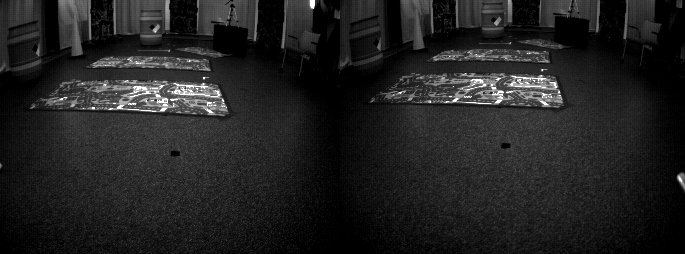
\includegraphics[width=\textwidth]{Codes/MVSEC/Hexacopterr.PNG}
        \caption{Stereowizyjne ujęcie z lotu drona ze4 zbioru danych MVSEC}
        \label{fig:MVSEC}
    \end{figure}
    
    
